\documentclass[tikz,border=2pt]{standalone}
\usepackage{amsmath,amssymb}
\usepackage{tikz}
\usetikzlibrary{matrix}

\begin{document}
% Testing the sign of Q(x) = x^T A x only on the subspace Bx = 0: form the bordered matrix
% H = [[0, B],[B^T, A]] and read the signs of its last n - m leading principal minors.
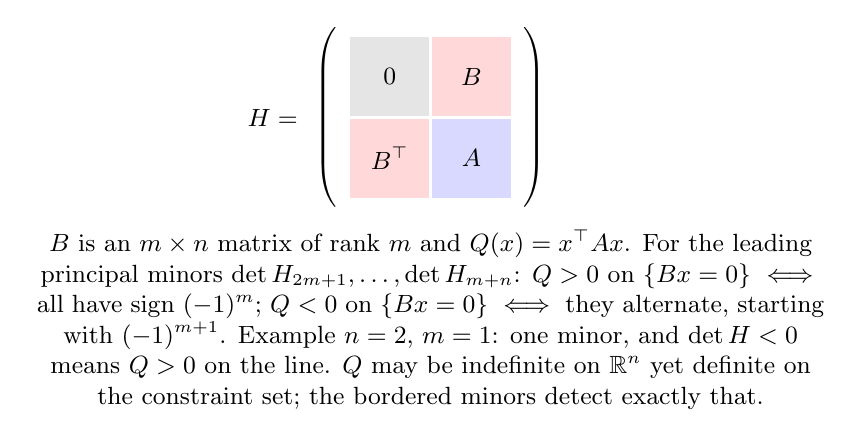
\begin{tikzpicture}[every node/.style={font=\small}]
	\matrix (H) [matrix of math nodes, nodes={minimum size=1.0cm, anchor=center}, left delimiter=(, right delimiter=), column sep=1pt, row sep=1pt] at (0,0) {
		|[fill=gray!20]| 0 & |[fill=red!15]| B \\
		|[fill=red!15]| B^{\top} & |[fill=blue!15]| A \\
	};
	\node[anchor=east] at ([xshift=-12pt]H.west) {$H=$};
	\node[anchor=north, align=flush center, text width=10cm] at (0,-1.3) {$B$ is an $m\times n$ matrix of rank $m$ and $Q(x)=x^{\top}Ax$. For the leading principal minors $\det H_{2m+1},\dots,\det H_{m+n}$: $Q>0$ on $\{Bx=0\}$ $\iff$ all have sign $(-1)^m$; $Q<0$ on $\{Bx=0\}$ $\iff$ they alternate, starting with $(-1)^{m+1}$. Example $n=2$, $m=1$: one minor, and $\det H<0$ means $Q>0$ on the line. $Q$ may be indefinite on $\mathbb{R}^n$ yet definite on the constraint set; the bordered minors detect exactly that.};
\end{tikzpicture}
\end{document}
